\documentclass{article}

\usepackage[left=1in, right=1in, top=1in, bottom=1in]{geometry}

\usepackage{setspace}
\usepackage{fancyhdr}
\usepackage{hyperref}
\usepackage{amsthm}
\usepackage{amssymb}
\usepackage{multirow}
\usepackage{enumitem}
\usepackage{graphicx}
\usepackage{makecell}
\usepackage{booktabs}
\usepackage{titlesec}
\usepackage{amsmath}
\usepackage{pdfpages}
\usepackage{enumitem}

\setcounter{secnumdepth}{4}

\hypersetup{
    colorlinks=true,     
    urlcolor=magenta
}

\renewcommand{\qedsymbol}{\rule{0.7em}{0.7em}}

\newlength\tindent
\setlength{\tindent}{\parindent}
\setlength{\parindent}{0pt}
\renewcommand{\indent}{\hspace*{\tindent}}
\setlength{\parskip}{0em}

\newenvironment{blockquote}{%
  \par%
  \vskip1em
  \leftskip=2em\rightskip=2em%
  \noindent\ignorespaces}{%
  \par\vskip1em}

\newenvironment{blockquote2}{%
	\par%
	\vskip1em
	\leftskip=4em\rightskip=4em%
	\noindent\ignorespaces}{%
	\par\vskip1em}

\pagestyle{fancy}
\fancyhf{}
\fancyhead[LO]{STA5176}
\fancyhead[RO]{Kyle Ligon}
\fancyfoot[LO]{Chapter 8 and 9}
\fancyfoot[RO]{\thepage}
 
\renewcommand{\headrulewidth}{0.5pt}
\renewcommand{\footrulewidth}{0.5pt}

\begin{document}
\section*{Chapter 8 and 9 Homework}
\subsection*{Due 3-18-2018}
\subsubsection*{Problem 9.13}
\subsubsection*{ a) Assess ANOVA assumptions using the graph from PROC MIXED.}

In order to proceed with ANOVA, we must check for the following pieces:
\begin{itemize}[leftmargin=+.5in]
 	\item[$\bullet$] No obvious pattern in our Residual Scatterplot
	\item[$\bullet$] Normal shape to the Residual Histogram.
 	\item[$\bullet$] Residuals fit along the linear prediction of our Actual "Normality" to the Theoretical Normal Model.  
\end{itemize}
Since there is no readily see-able pattern in our residuals, our distribution is mound shaped despite collection of residuals near positive 1, and our Residuals fit the along the Q-Q plot(although, there may be evidence of a right skew), we will proceed with ANOVA to see if at least one mean is different.  

\subsubsection*{ b) Perform ANOVA to determine if there is a difference among the five weight-reducing agents, $\alpha$ = 0.05.} 
\begin{table}[ht]
\caption{ANOVA Table for Weight Loss Study}
\centering
\begin{tabular}{l c c c c c}
\hline\hline
Row Names & SS & df & MS & F & P-Value \\ [0.5ex] 
\hline
Treatments (T) & 61.618 & 4 & 15.4045 & 15.6805 & 4.16x$10^{-8}$ \\
Error (E) & 44.207 & 45 & 0.9824 & \\
Total & 105.825 & 49 &  \\ [1ex]
\hline
\end{tabular}
\label{table:nonlin}
\end{table}

Hypotheses:
\begin{blockquote}
$H_{0}$: $\mu_{a1}$ = $\mu_{a2}$ = $\mu_{a3}$ = $\mu_{a4}$ = $\mu_{s}$ \\
$H_{1}$: At least one mean is different.  
\end{blockquote}
Test Statistic:
\begin{blockquote}
F = 15.6805
\end{blockquote}
Rejection Region:
\begin{blockquote}
Reject $H_{0}$ if $F_{0} > F_{\alpha, 4, 45}$ \\
$F_{0.95, 4 , 45} = 5.72$
\end{blockquote}
Conclusion/Interpretation:
\begin{blockquote}
Since our $F_{0} > 5.72$, there is strong enough evidence to support rejecting the null hypothesis that the means are the same.  The data provided does suggest at least one mean is different from the rest.  
\end{blockquote}

\pagebreak

\subsubsection*{ c) Determine significantly different pairs using Tukey's W with $\alpha$ = 0.05}
\begin{blockquote}
To find which groups are different from each other, we will utilize Tukey's W to check which means are different from one another.  We will verify this by checking which one's p-values are less than 0.05 after using the TukeyHSD test on our ANOVA Model in R.  
\end{blockquote}
Conclusion/Interpretation
\begin{blockquote}
With our Tukey W test being run, the differences lie in the following means:
\end{blockquote}

\begin{itemize}[leftmargin=+0.5in]
	\item[$\bullet$] s differs with $a_{1}$, $a_{2}$, and $a_{4}$
	\item[$\bullet$] $a_{1}$ differs with $a_{3}$
\end{itemize}



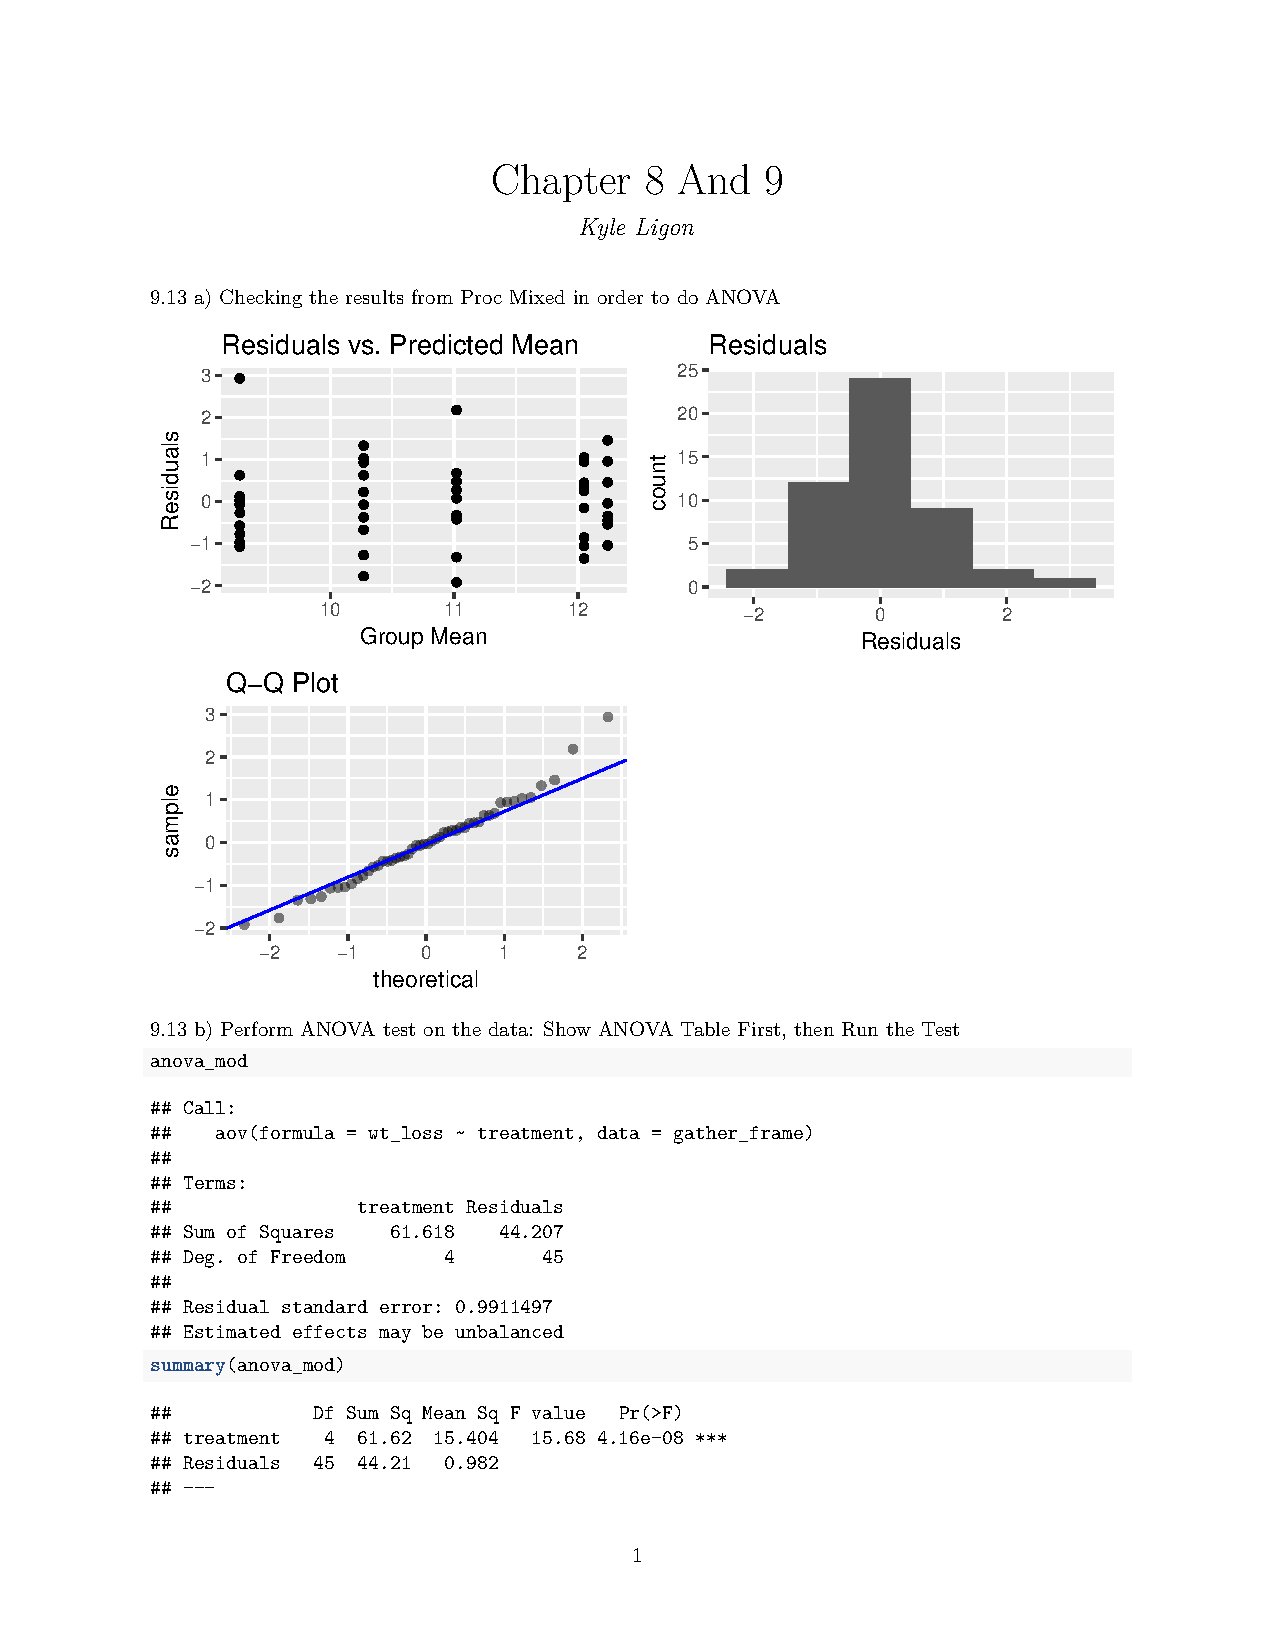
\includepdf[pages=-]{Chapter_8_And_9.pdf}
\end{document}



